\documentclass[]{standalone}
\usepackage[utf8]{inputenc}
\usepackage[american, siunitx]{circuitikz}
\usetikzlibrary{arrows,shapes,calc,positioning}

\usepackage{graphicx}

\newcommand{\myscope}[2] % #1 = name , #2 = rotation angle
{\draw[thick,rotate=#2] (#1) circle (12pt)
 (#1) ++(-0.35,-0.1) -- ++(0.3,0.3) --++(0,-0.3)-- ++(0.3,0.3) --++(0,-0.3);
}

\begin{document}

\pgfmathsetmacro\circuitheight{8}
\pgfmathsetmacro\circuitwidth{15}

\pgfmathsetmacro\ch{8}
\pgfmathsetmacro\cw{5}

\begin{circuitikz}[scale=1]
  % Power rails
  \draw (0, \circuitheight) to[V, label=24V] (0,0);
  \draw[red, thick] (0, \circuitheight) to[short, -o] ++(\circuitwidth, 0); 
  \draw[blue, thick] (0,0) to [short, -o] ++(\circuitwidth, 0); 


  \begin{scope}[xshift=11cm, yshift=2cm]
    \node at (0,0) {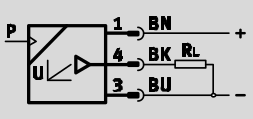
\includegraphics[width=3cm]{pressure-transmitter.png}};
    \node[coordinate] (psplus) at (1.2,.3) {};
    \node[coordinate] (psmin) at (1.2,-.4) {};
    \node[coordinate] (pssignal) at (2.6,-0.05) {};
    \draw (pssignal) to [short, -*] ++(-1.6,0);
  \end{scope}
  \draw (psplus |- 0,\circuitheight) to [short,-*] (psplus);
  \draw (psmin |- 0,0) to [short,-*] (psmin);
  \draw (pssignal |- (0,0) to[sV, color=white, name=S] (pssignal);
  \myscope{S}{0}

  \begin{scope}[xshift=10cm, yshift=6cm]
    \node[draw, minimum width=2cm, minimum height=1.6cm] (valve) at (0,0) {Valve};
    \node[coordinate, ] (vplus) at (-1.4, 0.6) {}; 
    \draw (valve.west |- vplus)  to [short, -*, color=red] (vplus);
    \node[coordinate, ] (vmin) at (-1.4, -0.6) {}; 
    \draw (valve.west |- vmin)  to [short, -*, color=blue] (vmin);
    \node[coordinate, ] (vwhite) at (-2.4, -0.2) {}; 
    \draw (valve.west |- vwhite)  to [short, -o] (vwhite);
    \node[coordinate, ] (vblack) at (-2.4, 0.2) {}; 
    \draw (valve.west |- vblack)  to [short, -*] (vblack);

  \end{scope}
  \draw (vplus |- 0,\circuitheight) to [short,] (vplus);
  \draw (vmin |- 0,0) to [short,] (vmin);
  \draw (vwhite |- 0,0) to [short,] (vwhite);


  \node[coordinate, left of=vblack, node distance=6.1cm] (Osc) {};
  \draw (vblack) to[short] (Osc) to[sV, color=white, name=S2] (Osc |- 0,0);
  \myscope{S2}{0}

  \begin{scope}[xshift=3cm, scale=0.5]
    \draw (0,\ch) to[american voltage source, a=10V] (0, 0); 
  
  \draw (0.5*\cw, \ch) to[R=$R_2$ ] (0.5*\cw, 0.5*\ch);
  \draw (\cw, \ch) to[R, l2=$R_1$ and \SI{68}{\ohm}] (\cw, 0.5*\ch);
  \draw (0.5*\cw, 0.5*\ch) to[push button] (\cw, 0.5*\ch);
  \draw (\cw, 0.5*\ch) to[R, l2=$R_3$ and \SI{47}{\ohm}] (\cw, 0);
  \draw (\cw, 0.5*\ch) to[short, -*] (1.5*\cw, 0.5*\ch) node[coordinate] (vdout) {};
  %\draw (0,0) to[short, -o] (1.5*\cw, 0);
  \draw (0, \ch) to[short] (\cw, \ch);
  %\draw (1.5*\cw, 0.5*\ch) to[european resistor, l=valve] (1.5*\cw, 0);

\end{scope}

\draw (vdout) |- (vblack);
\end{circuitikz}
\end{document}
